\section{Results}
\label{sec:results}
\begin{figure}
  \centering
  \subfloat[Uniform]{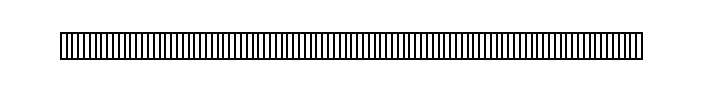
\includegraphics{adaptive_local_timestepping/images/mesh_uniform}}\\
  \subfloat[Polynomial]{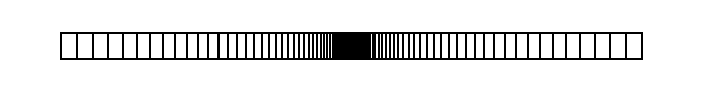
\includegraphics{adaptive_local_timestepping/images/mesh_polynomial}}\\
  \subfloat[Piecewise]{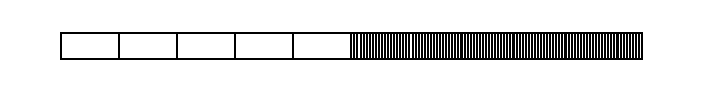
\includegraphics{adaptive_local_timestepping/images/mesh_piecewise}}
  \caption{Meshes used for numerical experiments}
  \label{fig:meshes}
\end{figure}

In this section we present results for the one dimensional Burgers' equation and the shallow water equations. Since the timestepping method is first order, we only consider first order finite volume schemes.
To demonstrate the robustness of the timestepping method for different types of meshes, we consider three meshes: a uniform mesh, a polynomial mesh, and a piecewise mesh. These meshes are generated by warping uniformly distributed nodes along $(-1,1)$ onto the interval $(-1,1)$. The base case is the uniform mesh for which the warp function is the identity, i.e. $w(x) = x$. The polynomial mesh refines the mesh around the origin. This type of mesh is common for finite element applications where local refinement is required to resolve flow around fine features. The warp function for this mesh is given as
\begin{equation*}
  w(x) = \frac{1}{1/3 + \varepsilon} \left( \frac{ x^3}{3} + \varepsilon x \right),
\end{equation*}
where we set $\varepsilon = 0.02$ in order the bound the ratio of largest to smallest cells. Lastly, we consider a mesh with a large jump in refinement. The warp function is then defined so that the ratios of cell sizes is at least 16 to 1. Assuming the nodes are enumerated $x_{j}$ for $0 \le j \le n_{el}$, define $j^*  = \lfloor n_{nodes}/17 \rfloor$. We then define the warp function for the piecewise mesh as
\begin{equation*}
  w(x) = \begin{cases}
    \frac{x + 1}{1 + x_{j^*}} - 1 & \text{for } j \le j^*\\
    \frac{x - 1}{1 - x_{j^*}} + 1 & \text{for } j > j^*\\
    \end{cases}.
\end{equation*}
For clarity the meshes used are depicted in Figure~\ref{fig:meshes}. To illustrate the behavior of the timestepping algorithm, we consider meshes with 100 cells and 20 submeshes in the next two sections.  In practice, the number of cells per submesh needs to be significantly larger to amortize runtime overheads with useful work. Section~\ref{sec:performance-results} showcases performance results with meshes consisting of 500,000 cells.

%additional performance considerations
%CFL condition


\subsection{Burgers' Equation}
Consider Burgers' equation on the line,
\begin{equation}
\partial_t u + \partial_x u^2/2 = 0.
\end{equation}
We consider two sets of initial conditions: firstly, the shockwave, which is initialized
\begin{equation*}
  u_0(x) = \begin{cases}
    1 & x < 0\\
    0 & x > 0,
    \end{cases}
\end{equation*}
and secondly a rarefaction wave,
\begin{equation*}
  u_0(x) = \begin{cases}
    -1 & x < 0\\
    1 & x > 0.
  \end{cases}
\end{equation*}

\begin{figure}
  \centering
  \subfloat[Uniform-Shockwave\label{fig:burgers:spacetime:uniform:shockwave}]{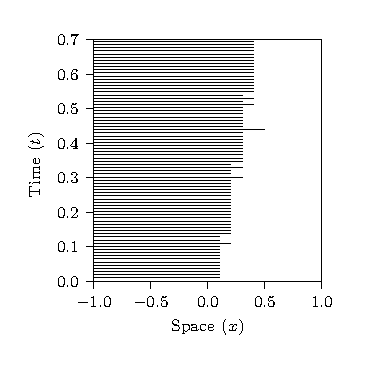
\includegraphics{{adaptive_local_timestepping/images/event_trace_burgers_uniform_shockwave}}}
  \hfill
  \subfloat[Uniform-Rarefaction\label{fig:burgers:spacetime:uniform:rarefaction}]{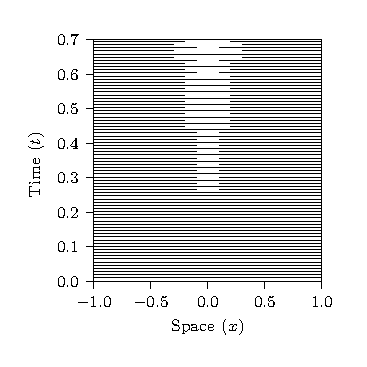
\includegraphics{{adaptive_local_timestepping/images/event_trace_burgers_uniform_rarefaction}}}
  \\
  \subfloat[Polynomial-Shockwave\label{fig:burgers:spacetime:polynomial:shockwave}]{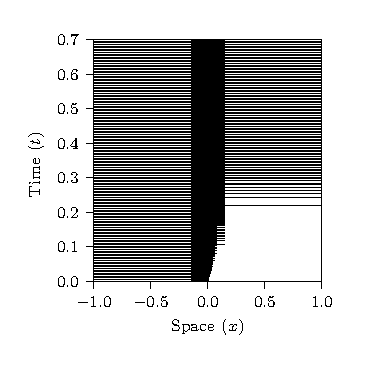
\includegraphics{{adaptive_local_timestepping/images/event_trace_burgers_polynomial_shockwave}}}
  \hfill
  \subfloat[Polynomial-Rarefaction\label{fig:burgers:spacetime:polynomial:rarefaction}]{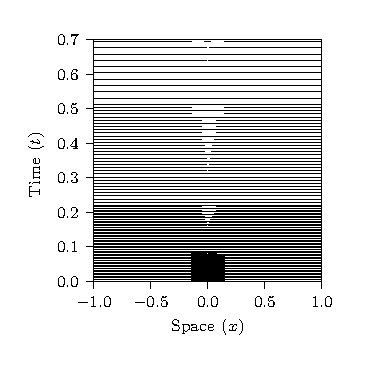
\includegraphics{{adaptive_local_timestepping/images/event_trace_burgers_polynomial_rarefaction}}}
  \\
  \subfloat[Piecewise-Shockwave\label{fig:burgers:spacetime:piecewise:shockwave}]{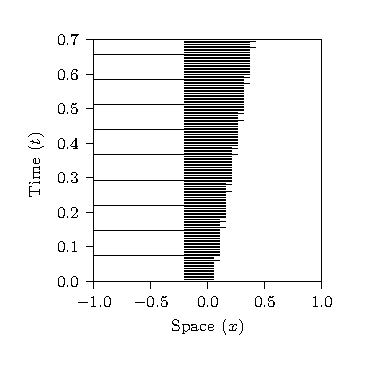
\includegraphics{{adaptive_local_timestepping/images/event_trace_burgers_piecewise_shockwave}}}
  \hfill
  \subfloat[Piecewise-Rarefaction\label{fig:burgers:spacetime:piecewise:rarefaction}]{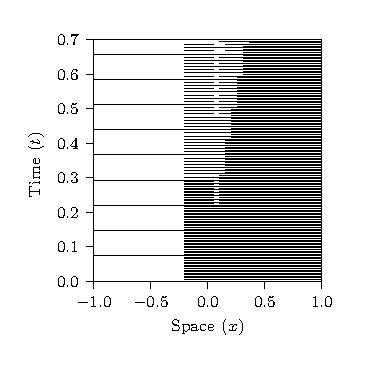
\includegraphics{{adaptive_local_timestepping/images/event_trace_burgers_piecewise_rarefaction}}}
  \caption{Space-time plots for Burgers' equation with various meshes and problem configurations.}
  \label{fig:burgers:spacetime}
\end{figure}


For both cases, we enforce the boundary conditions by setting the boundary value to the analytic solution. We note that these test cases highlight the ability of the local timestepping algorithm to refine the timestep---in the case of the shockwave---and the ability to coarsen the timestep---in the case of the rarefaction. To visualize the timesteps taken by these algorithms, we present space-time event traces similar to those shown in Figure~\ref{fig:sol-cartoon}. In these plots, the $x$-axis corresponds to the domain $\Omega$, and the $y$-axis represents simulation time, each line corresponds to an update having executed at that given time. The space-time plots are shown in Figure~\ref{fig:burgers:spacetime}.  For the shockwave and rarefaction problems on the uniform polynomial mesh, the $L^1$- and $L^2$-errors are bounded by 0.055. For the piecewise mesh, the errors are bounded by 0.15. Nevertheless, results for the piecewise mesh remain stable and show that the under resolved region is able to step with much larger timesteps. Looking at Figures~\ref{fig:burgers:spacetime:uniform:shockwave} and \ref{fig:burgers:spacetime:piecewise:shockwave}, we see that submeshes only update behind the shock front. For the shockwave initial conditions on the polynomial mesh---shown in Figure~\ref{fig:burgers:spacetime:polynomial:shockwave}---after $t=0.2$ the entire mesh begins stepping. This is due to the fact that cells in the interval $(0.146, 1)$ belong to a single submesh. Since these cells take larger timesteps the submesh partitioner places more cells into this submesh. In later results with more cells and submeshes, the inactive regions of the polynomial mesh do not update.
For the rarefaction problem, due to timestep binning, timestep coarsening happens only once the submesh is able to take a timestep twice as large as the previous timestep. 
For the analytic solution to the rarefaction wave at $t=0.7$--the end of the simulation---$|u|<0.5$ for $|x|<0.35$. This is consistent with the observed timestep  coarsening seen in Figure~\ref{fig:burgers:spacetime:uniform:rarefaction}. Similarly, the polynomial and piecewise meshes are able to adapt their timesteps appropriately. In these cases, the submesh partitions are not symmetric about $x=0$, giving rise to the asymmetry in the event traces.
 %\Cy{Consider adding a little more discussion about the Figures.  What should the reader be looking for and learning from them as you compare across mesh geometry and boundary conditions?}


\subsection{Shallow Water Equations}
In order to show that the local timestepping scheme is robust for more non-linear problems and in the absence of the theoretical guarantees, we provide two problems for the shallow water equations. Consider the system of conservation laws,
\begin{equation*}
  \begin{cases}
    \partial_t h + \partial_x q_x = 0 &\\
    \partial_t q_x + \partial_x ( hu^2 + gh^2/2) = -gh\partial_x z&\\
  \end{cases}
\end{equation*}
where $q_x = hu$, $z$ is the bathymetry, and $g=1$. We consider here the dam break Riemann problem, for which,
\begin{align*}
  h_0(x) &= \begin{cases}
    1 & \text{if } x < 0,\\
    1/16.1 & \text{if } x > 0,
  \end{cases}\\
  q_{x,0}(x) &= 0,\\
  z &= 0.
\end{align*}
For the shallow water equations the maximum advection speed, $|\Lambda|$ is  $\sqrt{gh} + |u|$. The initial conditions have been chosen to allow a 4-to-1 timestepping ratio between downstream and upstream of the dam break for the uniform mesh. The second shallow water test case we consider is the analytic problem of Carrier and Greenspan~\cite{Carrier1958}. This problem considers water moving up and down a shoreline with uniform slope in a periodic manner. We follow the set-up outlined in~\cite{Bokhove2005} with a phase shift of $\varphi=-\pi$.

For the numerical discretization, we use a local Lax-Friedrichs flux along with the first-order local hydrostatic reconstruction proposed in~\cite{Audusse2004}. The space time plots are shown in Figure~\ref{fig:swe:spacetime}.  We note that for the shallow water flow, the theoretical guarantees no longer hold. In fact, the timestepping region between the two waves emanating from the dam break problem in Figure~\ref{fig:swe:spacetime:uniform:dambreak} requires a finer timestep than observed during the beginning of the simulation, and thereby violates the progress guarantee, Lemma~\ref{lem:progress-guarantee}. For the dam break problem, the refinement of the timesteps looks similar to that of the shockwave problem for Burgers' equation. For the uniform and piecewise meshes, we see expected refining of timestep sizes, and for the polynomial mesh, regions far from the shock waves prematurely begin taking fine timesteps due to the large submeshes generated by the submesh partitioner.

For the Carrier-Greenspan problem on the uniform mesh, shown in Figure~\ref{fig:swe:spacetime:uniform:cg}, we see the wave moving in and out of the domain. Analytically, the water front never goes past $x=0.25$, and the simulated event trace reflects this as no submesh updates occur for in regions for which $x>0.3$.  For the polynomial mesh in Figure~\ref{fig:swe:spacetime:polynomial:cg}, we again begin stepping everywhere due to the submesh graph partitioning. For both of these cases, we note hysteretic effects in regions which are mesh drying. The final simulation time of $2 \pi$ contains two periods of the Carrier-Greenspan solution. At time $\pi$,  the submeshes participating in updates would ideally look identical to the start of the simulation, i.e. only submeshes which contain cells located at $x<-0.25$ would update. Rather we see this slow ``draining'' of mass as submeshes try to coarsen their timesteps, resulting in updates occurring in regions of the mesh that are dry in the analytic solution. The impact of behavior on performance will be touched upon in the next section. For the piecewise mesh, the incoming wave is so under resolved that it is unable to cause significant wetting and drying on the beach. Hence, this configuration fails to reproduce the periodic wetting and drying event trace seen for the uniform and polynomial meshes.

To conclude, the proposed timestepping method remains stable for simulations with dramatic temporal variations in $\Lambda$ as shown for Burgers' equation in Figure~\ref{fig:burgers:spacetime} and the shallow water equations in Figure~\ref{fig:swe:spacetime}. For the latter problem, we fail to satisfy the assumptions for the proof of correctness and even observe a violation of the progress guarantee, and yet the algorithm is able to stably compute the correct solution. Important in both problems is the ability for the algorithm to locally refine or coarsen timesteps. The proposed formulation dispenses with complicated book keeping relating to which timestepping level submeshes are in and how to appropriately define buffer zones, but simply computes and adjusts the timestep based on locally available information.


%\Cy{Again, a little more discussion would be nice.  Maybe point out advantages and disadvantages of the different mesh geometries for the different problems?}
\begin{figure}
  \centering
  \subfloat[Uniform-Dam break\label{fig:swe:spacetime:uniform:dambreak}]{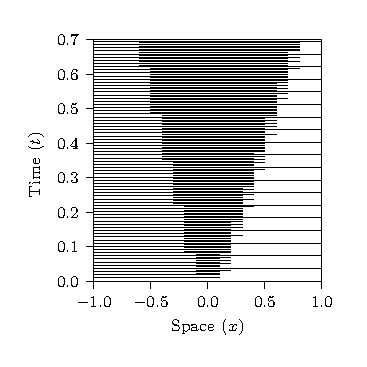
\includegraphics{{adaptive_local_timestepping/images/event_trace_swe_uniform_dambreak}}}
  \hfill
  \subfloat[Uniform-Carrier-Greenspan\label{fig:swe:spacetime:uniform:cg}]{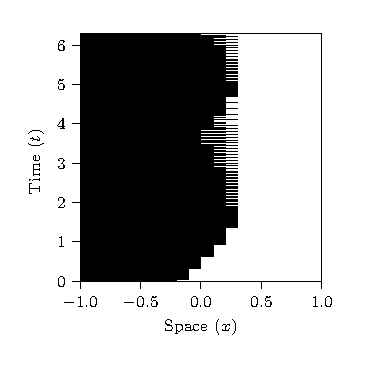
\includegraphics{{adaptive_local_timestepping/images/event_trace_swe_uniform_carrier-greenspan}}}
  \\
  \subfloat[Polynomial-Dam break\label{fig:swe:spacetime:polynomial:dambreak}]{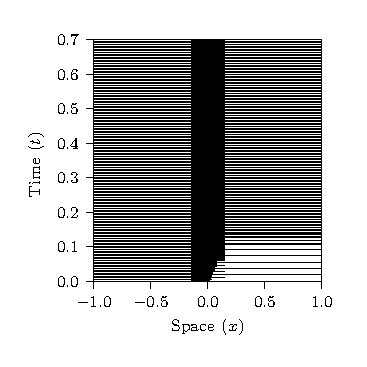
\includegraphics{{adaptive_local_timestepping/images/event_trace_swe_polynomial_dambreak}}}
  \hfill
  \subfloat[Polynomial-Carrier-Greenspan\label{fig:swe:spacetime:polynomial:cg}]{\includegraphics{{adaptive_local_timestepping/images/event_trace_swe_polynomial_carrier-greenspan}}}
  \\
  \subfloat[Piecewise-Dam break\label{fig:swe:spacetime:piecewise:dambreak}]{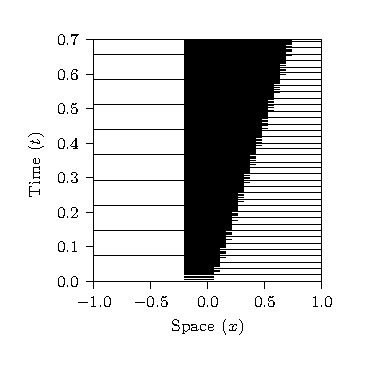
\includegraphics{{adaptive_local_timestepping/images/event_trace_swe_piecewise_dambreak}}}
  \hfill
  \subfloat[Piecewise-Carrier-Greenspan\label{fig:swe:spacetime:piecewise:cg}]{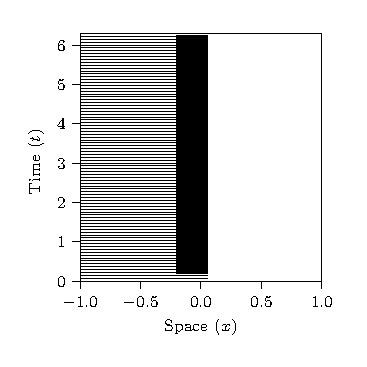
\includegraphics{{adaptive_local_timestepping/images/event_trace_swe_piecewise_carrier-greenspan}}}
  \caption{Space-time plots for the shallow water equations with various meshes and problem configurations.}
  \label{fig:swe:spacetime}
\end{figure}

\subsection{Performance Comparison}
\label{sec:performance-results}

In this section, we compare the performance of our local timestepping implementation to a flat MPI implementation. For the MPI implementation, we use non-blocking point to point messaging and hide message latencies with internal work. For more details, we refer the reader to implementation in~\cite{Bremer2019}. One key detail is that the MPI implementation does not compute the CFL condition, but rather uses a fixed timestep. Since dynamically updating a CFL condition would require an all-reduce at each timestep, the communication overhead makes an adaptive CFL condition non-viable for large-scale simulation. For the performance comparison, we consider the uniform and polynomial mesh with 500,000 cells on one Skylake node with 48 cores on TACC's Stampede2. A detailed overview of the computing environment as well as simulation parameters are presented in Appendix~\ref{sec:artifact}. We partition the mesh into 48 (one per core) uniform submeshes for the MPI implementation, and 288 (six per core) submeshes for the Devastator implementation based on the heuristic described in Section~\ref{sec:load-balancing}. %\Cy{may want to mention the reason for over-decomposition}
The over-decomposition factors of submeshes to ranks have been optimized for each runtime.
Over-decomposition of the mesh for Devastator enables three performance optimizations.
Firstly, over-decomposition allows a rank to hide message latencies. While one actor may be waiting on a message to arrive, the rank may execute events scheduled for other actors. 
Secondly, over-decomposition reduces the total amount of work required. Since each cell must step synchronously with other cells on that submesh, creating more submeshes implies that more cells are able to step with different timesteps. 
Lastly, more submeshes improves the performance of the load balancer. With more submeshes, the load balancing algorithm is able to more easily balance the simulation throughout all time points in the simulation. However, over-decomposition  comes at the cost of higher runtime overhead. More events with less work implies that a larger fraction of event execution time is spent on scheduling and control flow. The over-decomposition factor of 6 was chosen based on observed performance.
The MPI implementation does not benefit from over-decomposition. We explicitly hide message latencies by performing all internal work after posting sends and receives. Furthermore, the total number of cell updates---and thus work---remains independent of the over-decomposition factor and the load balancer is able to balance work across MPI ranks easily. 

To analyze the impact of the dynamic CFL condition versus the local timestepping due to mesh refinement, we consider two problems for the shallow water equations. Firstly, we consider a lake at rest problem, where
\begin{align*}
h_0(x) &= 1,\\
q_{x,0}(x) &= 0,\\
z &= 0.
\end{align*}
For this problem, differences in the CFL condition are solely a function of differences in cell size, $\Delta x$. The second problem we consider is the Carrier-Greenspan solution, outlined in the previous section. As the water front moves across the mesh, large portions of the mesh wet and dry throughout the simulation, causing these regions to experience large changes in allowable timestep sizes. For the lake at rest problem, the work in each submesh is approximately the same. Thus, we assign submeshes $[6\cdot k, 6 \cdot(k+1))$ to rank $k$. In the case of the Carrier-Greenspan problem, due to the periodic nature of $|\Lambda|$, we load balance over a quarter of the period, i.e. $\tend=\pi/2$ in~\eqref{eq:lb}. The performance data is shown in Table~\ref{tab:performance-data}. For the static uniform Lake at Rest problem, we include a Devastator configuration---labeled as (no CFL)---without the overhead of computing the local CFL in order to provide a more direct comparison with the MPI version, which does not compute the CFL in any configuration.  Each configuration is run 10 times with the average time elapsed, $\bar{T}$ reported in seconds. The standard deviation over the mean $\sigma_T/\bar{T}$ is given in percentages. Lastly, the number of updates and rollbacks are taken from a single run.  

We begin by noting that the number of cells rolled back is limited. At most 3.5\% of updates are rolled back suggesting that the performance related optimizations do a good job of preventing unnecessary rollback. The lack of rolled back updates for the uniform mesh lake at rest problem shows that we are able to completely avoid bad speculation for this configuration. For the lake at rest problem on the polynomial mesh, it should be possible to infer when messages are incoming since $|\Lambda|$ and $\Delta x$ are fixed. The existence of rollbacks implies that there is still future work to be done to prevent bad speculation.

\begin{table}
{\footnotesize
\caption{Execution times for the shallow water equations on Stampede2.}
\label{tab:performance-data}
  \centering
%This file is generated as part of a script. Instead of directly editing it
%please make the appropriate changes in images/src/raw_performance_data.py

\begin{tabular}{|c|c|c|c|c|c|c|c|c|} \hline
Problem & Mesh & Runtime & $\bar{T}$ & $\sigma_T/\bar{T}$ & $\#$ of Updates & $\#$ of Rollbacks\\\hline
Lake at Rest & Uniform & Devastator (no CFL) &  139.4 & 0.8\% & $252.5\cdot 10^9$ & 0 \\\hline
Lake at Rest & Uniform & Devastator &  173.2 & 0.8\% & $252.5\cdot 10^9$ & 0 \\\hline
Lake at Rest & Uniform & MPI &  133.2 & 0.1\% & $252.5\cdot 10^9$ & -- \\\hline
Lake at Rest & Polynomial & Devastator &  192.6 & 3.3\% & $239.7\cdot 10^9$ & $  3.5\cdot 10^9$ \\\hline
Lake at Rest & Polynomial & MPI &  478.4 & 2.0\% & $892.2\cdot 10^9$ & -- \\\hline
Carrier-Greenspan & Uniform & Devastator &  729.4 & 1.1\% & $856.2\cdot 10^9$ & $ 12.0\cdot 10^9$ \\\hline
Carrier-Greenspan & Uniform & MPI &  995.7 & 0.7\% & $1674.5\cdot 10^9$ & -- \\\hline
Carrier-Greenspan & Polynomial & Devastator & 3212.4 & 0.5\% & $3209.6\cdot 10^9$ & $113.3\cdot 10^9$ \\\hline
Carrier-Greenspan & Polynomial & MPI & 10732.0 & 0.1\% & $18070.1\cdot 10^9$ & -- \\\hline
\end{tabular}
}
\end{table}


\begin{table}
{\footnotesize
\caption{Theoretical versus observed speed-ups.}
\label{tab:speed-ups}
  \centering
\include{adaptive_local_timestepping/images/speedups}
}
\end{table}
The speed-up achieved via local timestepping is attained through work reduction. 
To assess the quality of our implementation, we contextualize execution times with configuration-dependent metrics to determine what fraction of unnecessary work was skipped. 
Recall the theoretical speed-up $S^{th}$, which estimates the maximum achievable speed-up based on analytic values of $\Lambda$ and $\Delta x$. We compare this theoretical estimate against a speed-up based on the number of cells updated.
 Let $W^{obs}_{MPI}$ and $W^{obs}_{deva}$ be the number of cells updated during the simulation with respective runtimes, and define the work-based speed-up as $S^{work}$ the ratio of observed updates, i.e.
\begin{equation*}
S^{work} = \frac{W^{obs}_{MPI}}{W^{obs}_{deva}}.
\end{equation*}
Discrepancies in $S^{work}$ and $S^{th}$ arise due to the enforcing of the local ordering constraint as well as extra updates arising from a combination of timestep binning and variations in $\Lambda$.

Lastly, we introduce the observed speed-up, which is based on the ratio of run times,
\begin{equation*}
S^{obs} = \frac{ \bar{T}_{MPI} }{\bar{T}_{deva}},
\end{equation*} 
where $\bar{T}_*$ corresponds to the mean observed execution time for either runtime. While the work based speed-up $S^{work}$ represents an upper bound on achievable speed-up, the observed speed-up is able to take into consideration factors such as imbalance, rollbacks, and algorithmic overhead.

Table \ref{tab:speed-ups} presents the three speed-up values for each configuration. The discrepancies between $S^{th}$ and $S^{work}$ are less than 3\% with the exception of the Carrier-Greenspan polynomial configuration where we over-predict the attainable speed-up by 17\%. In particular, we suspect these discrepancies result due to difficulties in water draining out of dry regions akin to the updates seen in Figures~\ref{fig:swe:spacetime:uniform:cg} and \ref{fig:swe:spacetime:polynomial:cg}.

 The observed speed-up ranges from $\minSObsOverWork\%$ to $\maxSObsOverWork\%$ of the work-based theoretical speed-up, $S^{work}$. 
 Since there is no theoretical benefit from using adaptive, local timestepping in the lake at rest on a uniform mesh configuration, this case highlights the overhead associated with using an adaptive, local timestepping scheme versus a static synchronous timestepping scheme. If we skip the CFL computation and use the analytic value of $K^{\intr}$ (see the first row of Table~\ref{tab:performance-data}), the observed speed-up is  $S^{obs}=\SobsNoCFL$. 

\begin{figure}
\centering
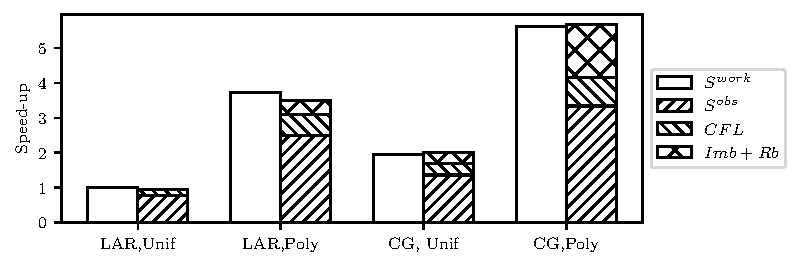
\includegraphics{{adaptive_local_timestepping/images/bar_plot_speed_ups}.pdf}
\caption{Comparison of speed-up due to work  reduction $S^{work}$ against observed speed-up $S^{obs}$ and the impact of avoiding CFL computations $(CFL)$ and fixing load imbalance and rollbacks $(Imb + Rb)$ for the lake at rest (LAR) and Carrier-Greenspan (CG) problem on the uniform (Unif) and polynomial meshes (Poly).}
\label{fig:imbalance-bars}
\end{figure}

To distinguish between algorithmic overhead of computing the CFL condition and other performance issues, we account for the cost of the CFL condition by multiplying the MPI execution times by the ratio of the execution times between the CFL and the no-CFL configurations of the lake at rest problem on the uniform mesh using the Devastator runtime. With these corrections, we obtain \effLARPoly{} of $S^{work}$ for the lake at rest problem with the polynomial mesh, \effCGUnif{} of $S^{work}$ of the Carrier-Greenspan problem with the uniform mesh, and \effCGPoly{} of $S^{work}$ of the Carrier-Greenspan problem for the polynomial mesh.
Furthermore, the impact of load imbalance and rollbacks is approximated by considering the average imbalance during the simulation. The imbalance is computed as the ratio of cells updated (both rolled back and committed) on the most overworked rank divided by the average number of committed cell updates across all ranks. Over a sufficiently small time interval this imbalance ratio approximates the improvement obtained through perfect load balancing. We estimate the impact of load imbalance by considering average imbalance over 100 evenly sized time intervals.

The cumulative performance impacts of the CFL computation and load imbalance are shown in Figure~\ref{fig:imbalance-bars}. This graph compares the speed-up due to work reduction, $S^{work}$ against the observed speed-up $S^{obs}$ and illustrates how the CFL computation and load imbalance account for the discrepancy. It is important to note that a given part of the stacked bar graph multiplies factors below it, e.g. the top of the $Imb+Rb$ bar corresponds to the expected speed-up if the simulation were perfectly balanced {\em and} there was no cost associated with the CFL condition. This distorts the size of bars towards the top of the graph, but allows us to compare the magnitudes of the speed-ups across problem configurations. With these two factors, we are able to account for the discrepancy in expected $S^{work}$ and observed $S^{obs}$ speed-ups within $\maxSpeedupErr\%$.

We also observed that rollback had a limited impact on performance for our experimental configurations.  For the Carrier-Greenspan problem, rollback minimally impacted the imbalance of the simulation with the imbalance metric increasing by no more than \imbCGdtRb{} for either mesh. For the polynomial lake at rest problem, the imbalance of committed updates was only \polynomialImb . However, once rollbacks are taken into consideration the imbalance went up to \polynomialImbwRb . Rollbacks are observed near regions of large CFL variation. For the Carrier-Greenspan problem, the lack of local clustering in the mapping of submeshes to ranks distributed rollbacks across ranks, and the impact of rollbacks on imbalance is relatively limited. However, for the polynomial lake at rest problem, each rank is assigned a contiguous chunk of submeshes, and rollback tends to aggregate on a few ranks.

Another cause of the performance degradation due to imbalance may be limitations of static load balancing. Firstly, there exist discrepancies between the performance model outlined in Section~\ref{sec:load-balancing} and the observed work done by each submesh, as evidenced by discrepancies between $S^{th}$ and $S^{work}$. Since the load balancing is based on the work of the theoretical model, this may lead to load imbalances, which we are not accounting for. Furthermore, the lower bound for the imbalance of the Carrier-Greenspan problem at the end of the Gurobi partitioning was 20\%. Although this lower bound does not account for the discrepancy between the performance model and observed work as well as error due to the quadrature used to approximate the integral in \eqref{eq:lb}, it suggests that there are underlying limits to how well the partitioner is able to statically load balance the problem. In that case, further reduction in load imbalance would benefit from dynamic load balancing techniques outlined in~\cite{Bremer2018}.

Lastly, we note that while the overhead associated with computing the CFL condition may seem high, it is worth noting that the MPI implementation is not provably stable. For the results presented here, we are able to take optimal timestep sizes, because we are able to analytically determine $(\Lambda / \delta x)_{\max}$. In practice, this value is unobtainable, and the selected $\Delta t$ would either lead to sub-optimal timestepping, i.e. taking timesteps smaller than necessary or manifest instabilities. The local timestepping algorithm can set an arbitrarily small $\Delta t_{\min}$,  and then take appropriately sized timesteps with step-size reductions taken as needed to guarantee stability.
